\section{Linux}
Nous supposerons que vous utilisez ubuntu et apt pour gestionnaire de paquets.


\subsection{Avec Network-manager}

Ouvrez Network-manager (nework connections).
\subsubsection{Challenge-MD5}
Ouvrez l'onglet Wired et ajoutez une nouvelle connection en cliquant sur 'Add'.\\
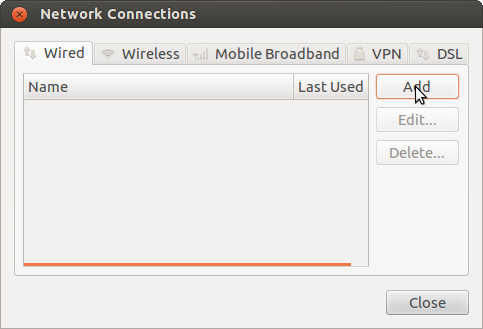
\includegraphics[width=\screenShotSize{}]{img/wiredAdd.png}\\
Dans l'onglet 'Wired' du nouveau panneau, choisissez votre MAC adresse dans le menu déroulant.\\
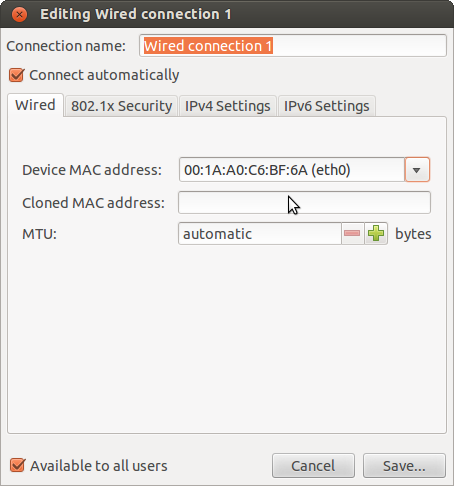
\includegraphics[width=\screenShotSize{}]{img/setMac.png}\\
Puis dans l'onglet 802.1x, cochez 'Utiliser la sécurtité 802.1x pour cette connexion'.\\
Sélectionnez MD5 dans le menu déroulant 'Authentification'. Enfin remplissez les champs 'Username' et 'Password'\\
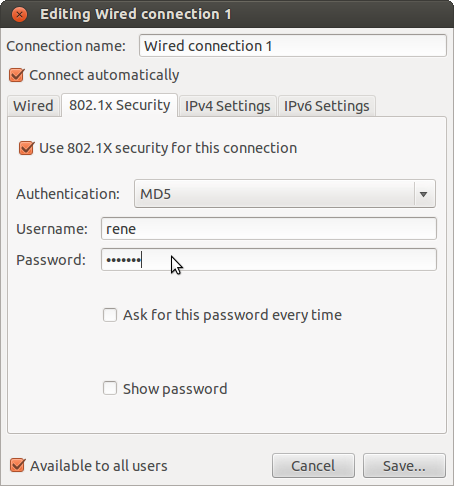
\includegraphics[width=\screenShotSize{}]{img/md5.png}\\
Cliquez ensuite sur 'sauvegarder' et fermez la fenêtre.
Il ne reste alors plus qu'à se connecter physiquement au réseau.


\subsubsection{PEAP}
Ouvrez l'onglet Wired et ajoutez une nouvelle connection en cliquant sur 'Add'.\\
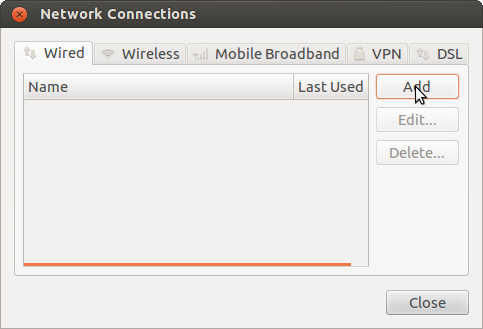
\includegraphics[width=\screenShotSize{}]{img/wiredAdd.png}\\
Dans l'onglet 'Wired' du nouveau panneau, choisissez votre MAC adresse dans le menu déroulant.\\
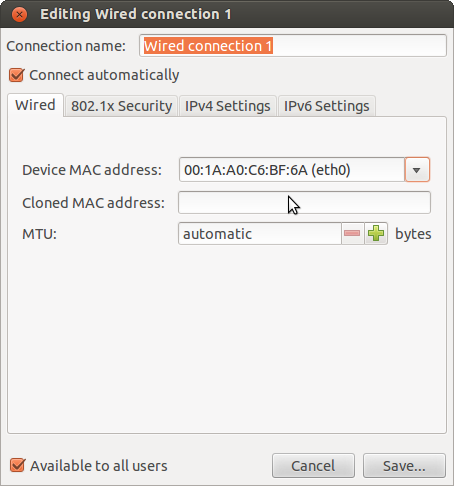
\includegraphics[width=\screenShotSize{}]{img/setMac.png}\\
Puis dans l'onglet 802.1x, cochez 'Utiliser la sécurtité 802.1x pour cette connexion'.\\
Sélectionnez 'Protected EAP (PEAP)' dans le menu déroulant 'Authentification'. 
Cliquez sur le bouton à coté de CA certificate et choisissez votre certificat racine.\\
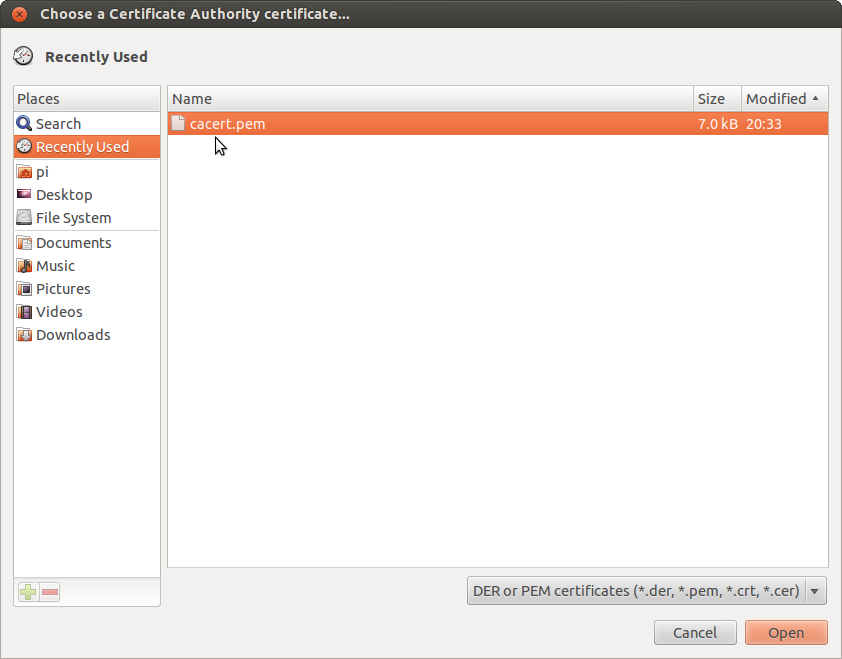
\includegraphics[width=\screenShotSize{}]{img/selectCacert.png}\\
Remplissez les champs 'Username' et 'Password'.\\
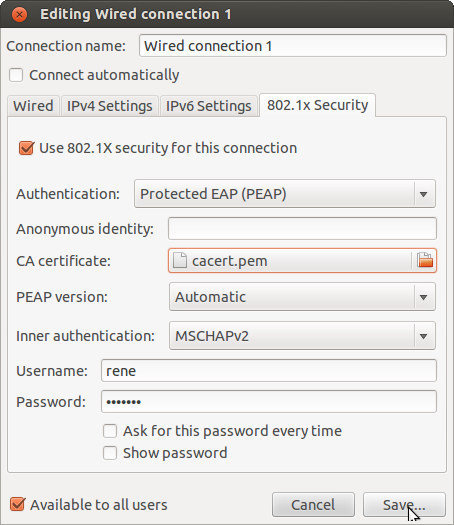
\includegraphics[width=\screenShotSize{}]{img/peap.png}\\
Cliquez ensuite sur 'sauvegarder' et fermez la fenêtre.
Il ne reste alors plus qu'à se connecter physiquement au réseau.\\

\subsubsection{TTLS}
Ouvrez l'onglet Wired et ajoutez une nouvelle connection en cliquant sur 'Add'.\\
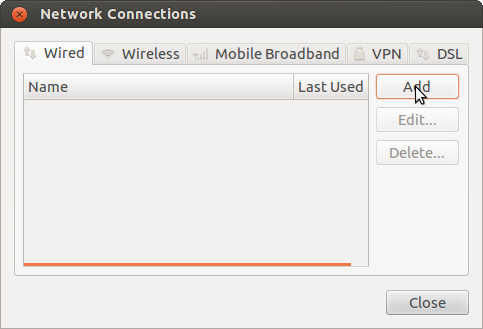
\includegraphics[width=\screenShotSize{}]{img/wiredAdd.png}\\
Dans l'onglet 'Wired' du nouveau panneau, choisissez votre MAC adresse dans le menu déroulant.\\
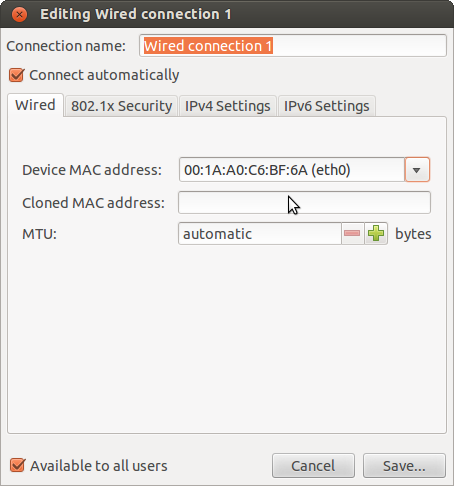
\includegraphics[width=\screenShotSize{}]{img/setMac.png}\\
Puis dans l'onglet 802.1x, cochez 'Utiliser la sécurtité 802.1x pour cette connexion'.\\
Sélectionnez 'Tunneled TLS' dans le menu déroulant 'Authentification'. 
Cliquez sur le bouton à coté de CA certificate et choisissez votre certificat racine.\\
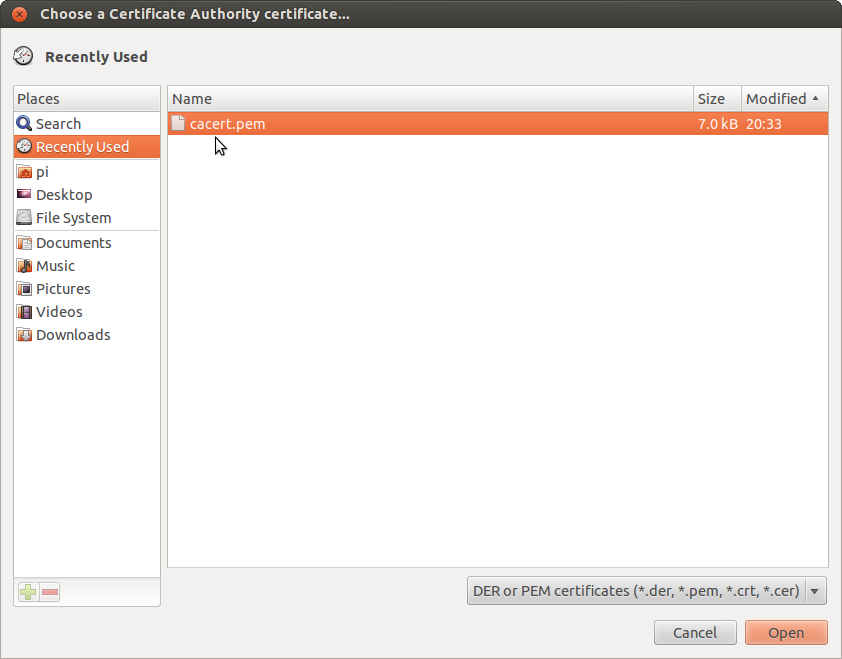
\includegraphics[width=\screenShotSize{}]{img/selectCacert.png}\\
Remplissez les champs 'Username' et 'Password'.\\
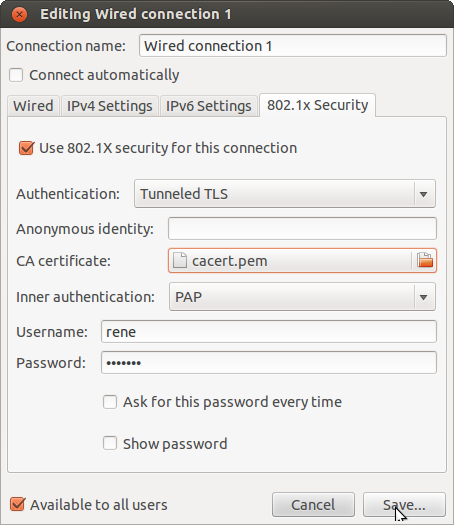
\includegraphics[width=\screenShotSize{}]{img/ttls.png}\\
Cliquez ensuite sur 'sauvegarder' et fermez la fenêtre.
Il ne reste alors plus qu'à se connecter physiquement au réseau.\\

\subsubsection{TLS}
Ouvrez l'onglet Wired et ajoutez une nouvelle connection en cliquant sur 'Add'.\\
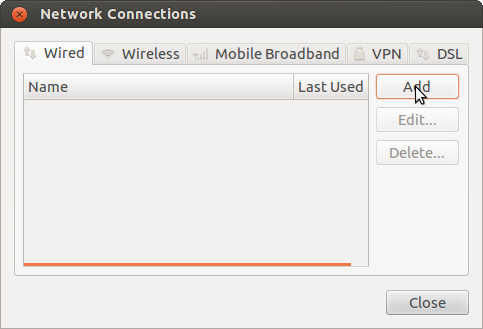
\includegraphics[width=\screenShotSize{}]{img/wiredAdd.png}\\
Dans l'onglet 'Wired' du nouveau panneau, choisissez votre MAC adresse dans le menu déroulant.\\
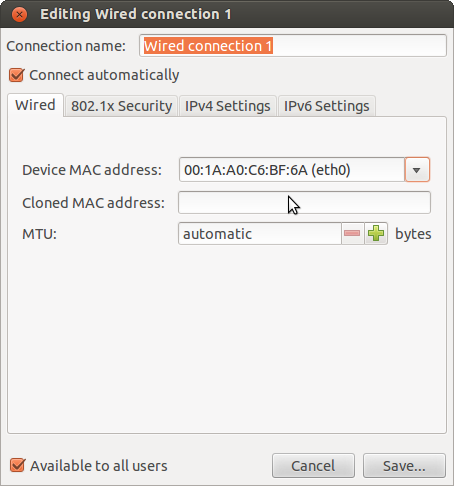
\includegraphics[width=\screenShotSize{}]{img/setMac.png}\\
Puis dans l'onglet 802.1x, cochez 'Utiliser la sécurtité 802.1x pour cette connexion'.\\
Sélectionnez 'TLS' dans le menu déroulant 'Authentification'. 
Cliquez sur le bouton à coté de CA certificate et choisissez votre certificat racine.\\
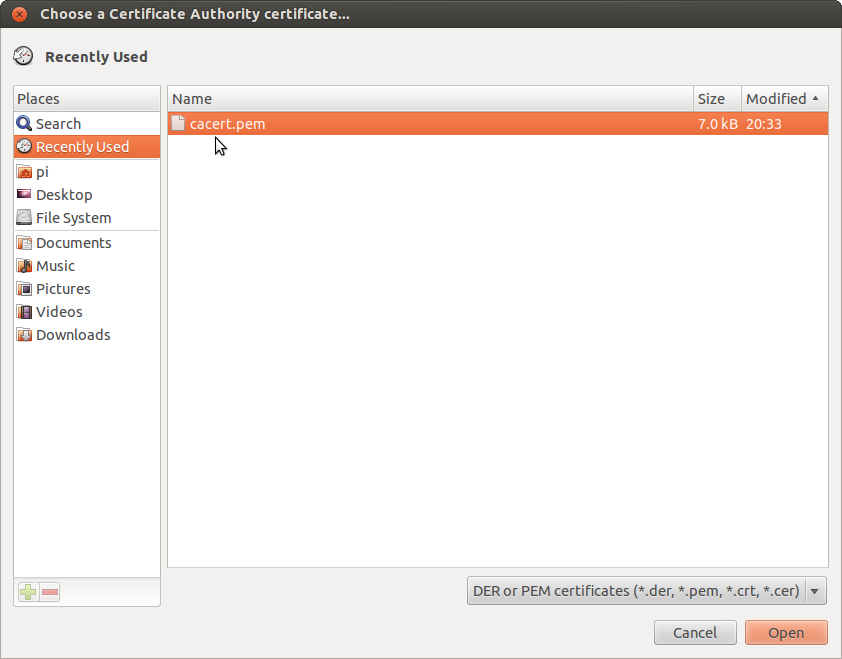
\includegraphics[width=\screenShotSize{}]{img/selectCacert.png}\\
Cliquez sur le bouton à coté de Private key et choisissez votre fichier p12.\\
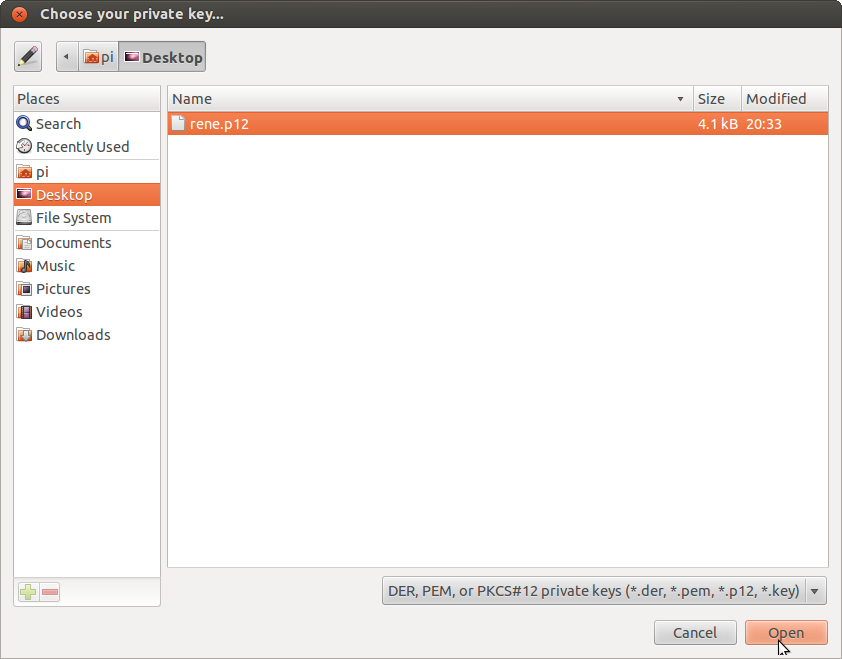
\includegraphics[width=\screenShotSize{}]{img/selectP12.png}\\
Cliquez sur le bouton à coté de User certificate et choisissez votre fichier pem.\\
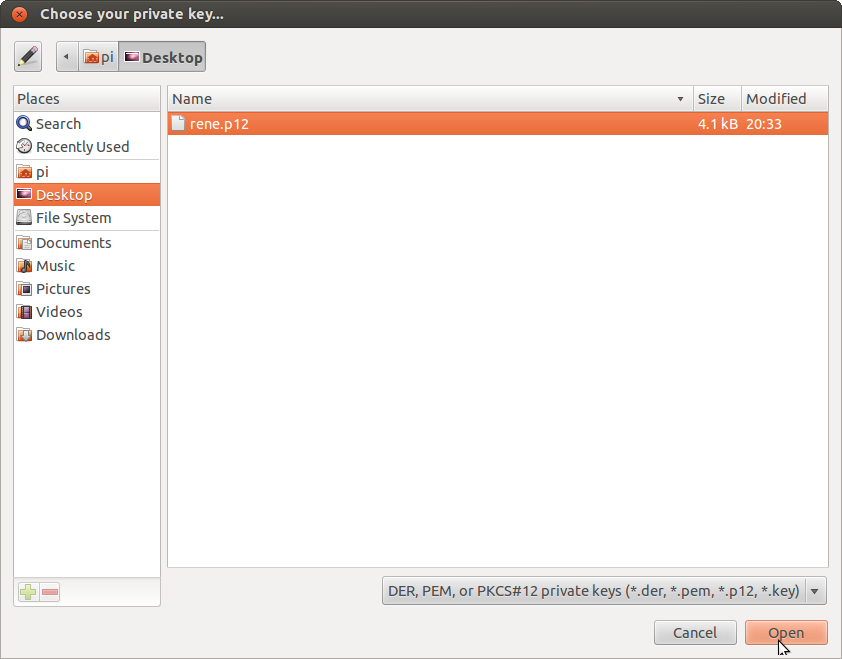
\includegraphics[width=\screenShotSize{}]{img/selectP12.png}\\
Remplissez le champs 'Username'.\\
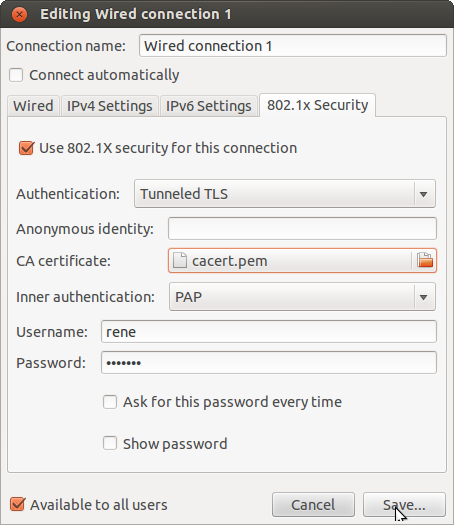
\includegraphics[width=\screenShotSize{}]{img/ttls.png}\\
Cliquez ensuite sur 'sauvegarder' et fermez la fenêtre.
Il ne reste alors plus qu'à se connecter physiquement au réseau.\\





\subsection{Avec wpa-supplicant}
Si vous ne l'avez pas déjà installé, installez wpa\_supplicant.
\begin{lstlisting}
$ sudo apt-get install wpa_supplicant
\end{lstlisting}
Il vous suffit alors d'utiliser un fichier l'un des fichier de configuration ci dessous.
Vous pouvez alors lancer wpa\_supplicant avec la commande suivante~:
\begin{lstlisting}
$ sudo wpa_supplicant -cpath/to/configuration/file.conf -ieth0 -Dwired -B
\end{lstlisting}


\subsubsection{Challenge-MD5}
\begin{lstlisting}
network={
        key_mgmt=IEEE8021X
        eap=MD5
        identity="utilisateur1"
        password="pass_utilisateur1"
}
\end{lstlisting}




\subsubsection{TLS}
\begin{lstlisting}
network={
    eap=TLS
    eapol_flags=0
    key_mgmt=IEEE8021X
    identity="utilisateur1"
    ca_cert="dossier_certs_utilisateur/cacert.pem"
    client_cert="dossier_certs_utilisateur/utilisateur1§§_cert.pem"
    private_key="dossier_certs_utilisateur/utilisateur1§§_key.pem"
}
\end{lstlisting}

Pour TLS, en utilsant un certificat au format p12~: 

\begin{lstlisting}
network={
    eap=TLS
    eapol_flags=0
    key_mgmt=IEEE8021X
    identity="utilisateur1"
    ca_cert="dossier_certs_utilisateur/cacert.pem"
    private_key="dossier_certs_utilisateur/utilisateur1.p12"
}
\end{lstlisting}

\subsubsection{TTLS}
Pour TTLS avec un chiffrement MD5 dans le tunnel~:

\begin{lstlisting}
network={
    eap=TTLS
    eapol_flags=0
    key_mgmt=IEEE8021X
    identity="utilisateur1"
    password="pass_utilisateur1"
    ca_cert="dossier_certs_utilisateur/cacert.pem"
    phase2="auth=MD5"
}
\end{lstlisting}

\subsubsection{PEAP}

Enfin, pour PEAP~:

\begin{lstlisting}
network={
    eap=PEAP
    eapol_flags=0
    key_mgmt=IEEE8021X
    identity="utilisateur1"
    password="pass_utilisateur1"
    ca_cert="dossier_certs_utilisateur/cacert.pem"
    phase2="auth=MSCHAPV2"
}
\end{lstlisting}



